%====================================================================================
\section[Poisson]{El modelo de regresión de Poisson}
%====================================================================================
\begin{frame}
	Principales caracter\'{i}sticas:
		\begin{itemize}
			\item El modelo Poisson está asociado a valores no negativos enteros (espacio $\mathbb{Z}$) de la variable dependiente, además de tener  una característica discreta y asociada a un conteo de casos.
			\item Por ejemplo, número de niños nacidos en el año; número de crímenes por semana; número de patentes por semana, número de casos Covid-19 en un día. 
		\end{itemize}
	El modelo Poisson puede expresarse en el valor esperado de la función exponencial:
		\begin{equation}\label{eqn:poiss}
			E(y|x_1,x_2, \dots, x_k)=\exp(\beta_0+\beta_1x_1+\dots+\beta_kx_k)
		\end{equation}
	Taking logs
		\begin{equation}
			\log (E(y|x_1,x_2, \dots, x_k))=\beta_0+\beta_1x_1+\dots+\beta_kx_k \equiv \boldsymbol{x\beta}
		\end{equation}
\end{frame}
%---------------------------------------------------
\begin{frame}{La función Log-likelihood}
	La función de distribución Poisson está definida por la probabilidad condicional en $\lambda$ para cada $h$:
		\begin{align*}
			P(Y=h | \lambda)=\frac{\exp(-\lambda)\lambda^h}{h!}
		\end{align*}
	Así modelamos en cambio la función de likelihood $P(y=h | \lambda)$
		\begin{align*}
			P(Y=h | \lambda)=\frac{\exp(-\exp(\boldsymbol{x\beta}))\exp(\boldsymbol{x\beta})^h}{h!}
		\end{align*}
	taking logs:
		\begin{align*}
			\log P(Y=h | \lambda)=-\exp(\boldsymbol{x\beta})+h \boldsymbol{x\beta}-\log (h!)
		\end{align*}
\end{frame}
%---------------------------------------------------
\begin{frame}{La función Log-likelihood}
	Considerando $h=y_i$ para una observación en particlar $i$.
		\begin{align*}
			\log P(Y=y_i | \lambda)=-\exp(\boldsymbol{x\beta})+y_i \boldsymbol{x\beta}-\log (y_i!)
		\end{align*}
	Sumando a través de las observaciones en la muestra:
		\begin{align*}
			L( \boldsymbol{\beta})=\sum_{i}^n\{y_i \boldsymbol{x\beta} - \exp(\boldsymbol{x\beta}) -\log (y_i!)\}
		\end{align*}
	Los parámetros contenidos en el vector $\beta$ se obtienen maximizando la función de log likelihood.
\end{frame}
%---------------------------------------------------
\begin{frame}{Partial effects}
	Calculando el porcentaje de cambio en el esperado condicional de $y$ dado un cambio en la variable $x$ (una semi-elasticidad):
		\begin{equation}
			\%\Delta (E(y|x_1,x_2, \dots, x_k))\approx100\beta \Delta x_j
		\end{equation}
	Siendo más precisos el cambio porcentual de $E(y|x)$ ante un cambio discreto en $x$
		\begin{equation}
			\Big(\frac{\exp(\beta_0+\beta_1x_1+\dots+\beta_k(c_k+1))}{\exp(\beta_0+\beta_1x_1+\dots+\beta_k(c_k))}-1\Big)\times 100 \equiv \Big(\exp(\beta_k)-1\Big) \times 100
		\end{equation}
	Donde el cambio discreto es igual a uno (1).
\end{frame}
%---------------------------------------------------
\begin{frame}{Partial effects}
	Se puede comparar los efectos parciales del modelo Poisson con el modelo logit y probit. Para esto se calcula $\frac{\partial E(y|x)}{\partial x_j} $ en la expresión (\ref{eqn:poiss}):
		\begin{align}
			\frac{\partial E(y|x)}{\partial x_j} =\exp(\beta_0+\beta_1x_1+\dots+\beta_kx_k) \beta_j
		\end{align}
	Tenemos que en el APE, el factor de escala es: $\sum_{i=1}^n \exp(\beta_0+\beta_1x_{i1}+\dots+\beta_kx_{ik}) $. Así entonces:
		\begin{align}
			\frac{\partial E(y|x)}{\partial x_j} =\overline{y}  \beta_j
		\end{align}
\end{frame}
%---------------------------------------------------
\begin{frame}{Important issue}
	Aunque el modelo Poisson es una elección natural para modelar datos de conteo. Tiene un ``important issue''.
		\begin{align}
			Var(y|x)=E(y|x)
		\end{align}
	En otras palabras es muy restrictivo. Aquí una pregunta de rigor: ?`Cuáles son las consecuencias? !`No muy serias! Si la distibución Poisson ``does o does not fit the data'', los $\beta$'s son aún consistentes y asintóticamente normal. Lo último es análogo al estimador OLS, el cual es consistente y asintóticamente normal si la suposición de normalidad se mantenga o no.
\end{frame}
%---------------------------------------------------
\begin{frame}{Important issue}
	Se puede hacer el modelo aún más flexible:
		\begin{align}
			Var(y|x)=\sigma^2 E(y|x)
		\end{align}
	El parámetro $\sigma^2$ es desconocido. Si $\sigma^2>1$ entonces existe evidencia que el proceso generador de datos tiene una varianza de ``overdispersion''; si $\sigma^2<1$ entonces la varianza tiene la característica de ``underdispersion''.
\end{frame}
%---------------------------------------------------
\begin{frame}{!Vayamos a STATA!}
	Exploremos la siguiente base de datos en la página de \href{http://fmwww.bc.edu/ec-p/data/wooldridge/datasets.list.html}{\textcolor{cyan}{Wooldridge}}. Utilizar el siguientes comando ``bcuse crime1''. Una descripción de las variables en la siguiente figura:
		\begin{figure}[htbp]
			\hspace*{+1cm} 
			\centering
				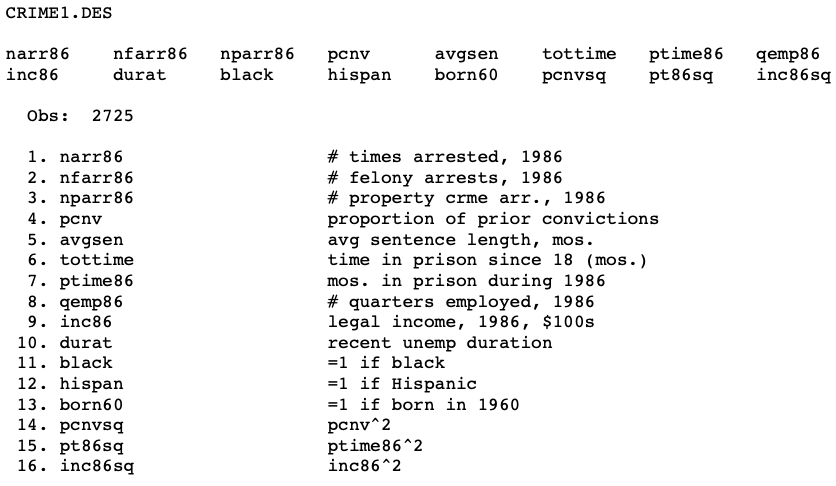
\includegraphics[width=0.63\linewidth]{fig/crime1} % requires the graphicx package
			\label{crime1}
			%  \caption{Source: own elaborati''}
		\end{figure} 
\end{frame}